\documentclass{article}

\usepackage{hyperref}
\usepackage{lipsum}
\usepackage{graphicx}
\usepackage[margin=0.9in]{geometry}
\usepackage{setspace}
\usepackage{mathtools}

\begin{document}

\begin{center}
\section*{Materials Science Lab 3 - Inductance}
\subsection*{Bijan Varjavand}
\end{center}

Inductance

\clearpage
\begin{center}
\section*{Materials Science Lab 3 - Meissner Effect}
\subsection*{Bijan Varjavand}
\end{center}

Resistance is a principal electronic property of materials. The classic equation for resistance is Ohm's Law, relating voltage, current, and resistance. However, this conventional understanding of resistance is insufficient when materials are put under.

93K is the literature value for critical superconducting temperature YBCO. 110K is the literature value for critical superconducting temperature BSCCO.

\begin{figure}[h!]
\centering
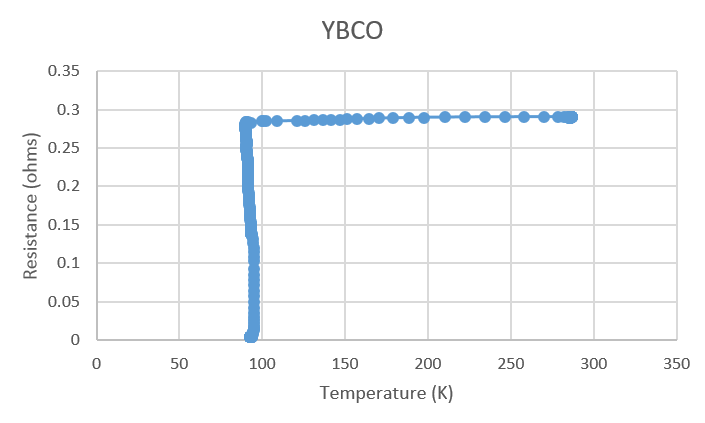
\includegraphics[scale=0.4]{YBCO.png}
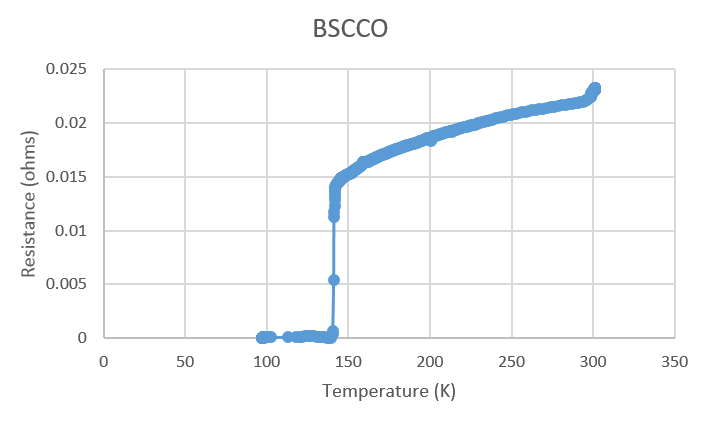
\includegraphics[scale=0.4]{BSCCO.png}
\end{figure}

\clearpage
\begin{center}
\section*{Materials Science Lab 3 - Hall Effect}
\subsection*{Bijan Varjavand}
\end{center}

WOWOWOWOWOWOWOWOOWO!

\clearpage
\section*{Sources}
$https://www.chemistryworld.com/$\\
$global-sei.com/$
\end{document}